\documentclass{beamer}

\usepackage[utf8]{inputenc}
\usepackage{tikz}
\usepackage{amsmath}
\usepackage{braket}
\usepackage{amsfonts}

\newtheorem{innercustomthm}{Postulate}
\newenvironment{Thm:Postulate}[1]
  {\renewcommand\theinnercustomthm{#1}\innercustomthm}
  {\endinnercustomthm}

\newcommand{\apparatus}[4]{\node[square node] (#1) at (#2,#3){#4};
                             \node[port] (#1+) at (#2 + 0.375, #3 + 0.5){+};
                             \node[port] (#1-) at (#2 + 0.375, #3 - 0.5){-};}

\setbeamertemplate{footline}[frame number]

%Information to be included in the title page:
\title{The consistent histories approach to the Stern-Gerlach experiment}
\author{Ian Wilson}
\institute{Oregon State University}
\date{June 2020}

\begin{document}

\frame{\titlepage}

\begin{frame}
\frametitle{The Stern-Gerlach (SG) Experiment}

\begin{figure}
\includegraphics[width=0.7\textwidth]{Figure-stern}
\caption{Otto Stern's original schematic (1922)}
\end{figure}

\begin{figure}
\includegraphics[width=0.4\textwidth]{Figure-new-stern}
\caption{Adapted from a modern analysis of the experiment by Rodríguez et al. (2016)}
\end{figure}
\end{frame}

\begin{frame}
\frametitle{Results of the SG Experiment}
\begin{itemize}
  \item Spin angular momentum is quantized
  \item Complementary physical variables
\end{itemize}
\begin{figure}
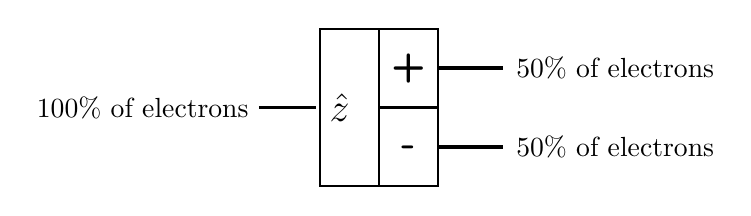
\begin{tikzpicture}[shorten >=1pt,auto, thick,
     square node/.style={rectangle, minimum height=2cm, minimum width=1.50cm, text width = 1.25cm, draw, font=\sffamily\Large\bfseries},
     port/.style={rectangle, draw,  minimum height=1cm, minimum width=0.75cm, font=\sffamily\Large\bfseries},
     wf/.style={rectangle, minimum height=1cm}]
    \apparatus{1}{2}{0}{$\hat{z}$};

    \node(w0) at (-1,0) {$100 \%$ of electrons};
    \node[wf] (w1) at (5, 0.5) {$50 \%$ of electrons};
    \node[wf] (w2) at (5, -0.5) {$50 \%$ of electrons};

    % \node(label1) at (0, -1.75) {$\bm{t_0}$};
    % \node(label2) at (6.25, -1.75) {$\bm{t_1}$};

    \draw[line width=0.5mm] (w0) -- (1);
    \draw[line width=0.5mm] (1+) -- (w1);
    \draw[line width=0.5mm] (1-) -- (w2);
\end{tikzpicture}
\end{figure}

\begin{figure}
\includegraphics[width=1.1\textwidth]{Figure-125}
\end{figure}

\end{frame}

\begin{frame}
\frametitle{Standard approach}

\begin{figure}
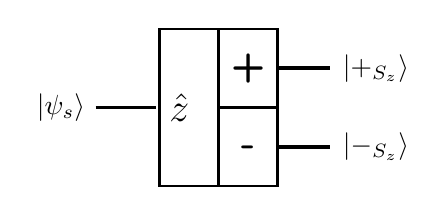
\begin{tikzpicture}[shorten >=1pt,auto, thick,
     square node/.style={rectangle, minimum height=2cm, minimum width=1.50cm, text width = 1.25cm, draw, font=\sffamily\Large\bfseries},
     port/.style={rectangle, draw,  minimum height=1cm, minimum width=0.75cm, font=\sffamily\Large\bfseries},
     wf/.style={rectangle, minimum height=1cm}]
    \apparatus{1}{2}{0}{$\hat{z}$};

    \node(w0) at (0,0) {$\ket{\psi_s}$};
    \node[wf] (w1) at (4, 0.5) {$\ket{+_{S_z}}$};
    \node[wf] (w2) at (4, -0.5) {$\ket{-_{S_z}}$};

    % \node(label1) at (0, -1.75) {$\bm{t_0}$};
    % \node(label2) at (6.25, -1.75) {$\bm{t_1}$};

    \draw[line width=0.5mm] (w0) -- (1);
    \draw[line width=0.5mm] (1+) -- (w1);
    \draw[line width=0.5mm] (1-) -- (w2);
\end{tikzpicture}
\end{figure}

\begin{itemize}
  \item Foundational assumptions are made about measurement
  \item Eigenvalues for operator variables are ``measurement results''
  \item Born rule assigns probabilities to the frequency of ``measurement results''
  \item State collapse prescribes special non-deterministic dynamics upon ``measurement''
  \item Dependent on ill-defined ``classical observer''
\end{itemize}
\end{frame}

\begin{frame}
  \frametitle{Motivating the removal of state collapse}

  \begin{itemize}
    \item Ambiguity of ``classical observer'' makes quantum mechanics vulnerable to pseudoscience
    \item Quantum mechanics is limited to predictions involving classical observers
    \item State collapse is asymmetric in time
  \end{itemize}

  \bigskip \bigskip

How can we describe the Stern-Gerlach experiment without postulating state collapse?
\end{frame}

\begin{frame}
\frametitle{Unitary measurement}
  \begin{itemize}
    \item Measurement can be described by the Schrödinger equation
    \item We begin by formalizing the spin-position interaction
  \end{itemize}
  \begin{figure}
    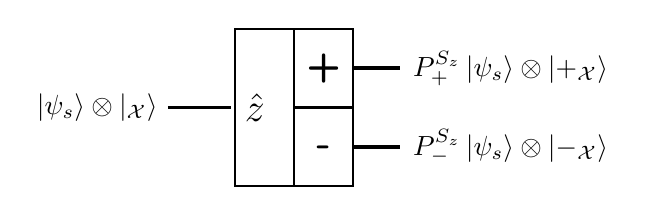
\begin{tikzpicture}[shorten >=1pt,auto, thick,
         square node/.style={rectangle, minimum height=2cm, minimum width=1.50cm, text width = 1.25cm, draw, font=\sffamily\Large\bfseries},
         port/.style={rectangle, draw,  minimum height=1cm, minimum width=0.75cm, font=\sffamily\Large\bfseries},
         wf/.style={rectangle, minimum height=1cm}]
        \apparatus{1}{2}{0}{$\hat{z}$};

        \node(w0) at (-0.5,0) {$\ket{\psi_s} \otimes \ket{\varnothing_\mathcal{X}}$};
        \node[wf] (w1) at (4.75, 0.5) {$P^{S_z}_+\ket{\psi_s} \otimes \ket{+_{\mathcal{X}}}$};
        \node[wf] (w2) at (4.75, -0.5) {$P^{S_z}_-\ket{\psi_s} \otimes \ket{-_{\mathcal{X}}}$};

        % \node(label1) at (0, -1.75) {$\bm{t_0}$};
        % \node(label2) at (6.25, -1.75) {$\bm{t_1}$};

        \draw[line width=0.5mm] (w0) -- (1);
        \draw[line width=0.5mm] (1+) -- (w1);
        \draw[line width=0.5mm] (1-) -- (w2);
    \end{tikzpicture}
  \end{figure}
  $P^{S_z}_\pm = \ket{\pm}\bra{\pm}$ is the projection operator for the $\ket{\pm}_{S_z}$ state.

\begin{align*}
    U(t_1, t_0)\ket{\psi_s}  =  P^{S_z}_+ \ket{\psi_s} \otimes \ket{+_{\mathcal{X}}} \: + \: P^{S_z}_- \ket{\psi_s} \otimes \ket{-_{\mathcal{X}}}
\end{align*}

\end{frame}

\begin{frame}
  \frametitle{Interaction with the environment}
  \begin{itemize}
    \item Newton's third law requires that the electron exerts a force on the magnet
    \item The ``environment'' includes all systems other than the electron (including the magnet)
  \end{itemize}
  \begin{figure}
  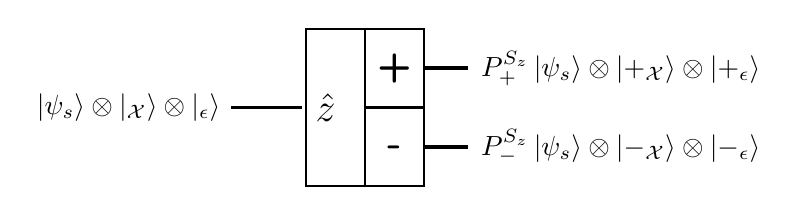
\begin{tikzpicture}[shorten >=1pt,auto, thick,
       square node/.style={rectangle, minimum height=2cm, minimum width=1.50cm, text width = 1.25cm, draw, font=\sffamily\Large\bfseries},
       port/.style={rectangle, draw,  minimum height=1cm, minimum width=0.75cm, font=\sffamily\Large\bfseries},
       wf/.style={rectangle, minimum height=1cm}]
      \apparatus{1}{2}{0}{$\hat{z}$};

      \node(w0) at (-1,0) {$\ket{\psi_s} \otimes \ket{\varnothing_\mathcal{X}} \otimes \ket{\varnothing_\epsilon}$};
      \node[wf] (w1) at (5.25, 0.5) {$P^{S_z}_+\ket{\psi_s} \otimes \ket{+_{\mathcal{X}}} \otimes \ket{+_\epsilon}$};
      \node[wf] (w2) at (5.25, -0.5) {$P^{S_z}_-\ket{\psi_s} \otimes \ket{-_{\mathcal{X}}} \otimes \ket{-_\epsilon}$};

      % \node(label1) at (0, -1.75) {$\bm{t_0}$};
      % \node(label2) at (6.25, -1.75) {$\bm{t_1}$};

      \draw[line width=0.5mm] (w0) -- (1);
      \draw[line width=0.5mm] (1+) -- (w1);
      \draw[line width=0.5mm] (1-) -- (w2);
    \end{tikzpicture}
  \end{figure}

  \begin{align*}
  U(t_1, t_0) &= \left(P^{S_z}_+ \otimes \mathcal{S}^\mathcal{X}_{\varnothing, +} \otimes \mathcal{S}^\epsilon_{\varnothing, +} \right) + \left(P^{S_z}_- \otimes \mathcal{S}^\mathcal{X}_{\varnothing, -} \otimes \mathcal{S}^\epsilon_{\varnothing, -} \right)
\end{align*}


\end{frame}

\begin{frame}
  \frametitle{Environment as a record keeper}
  \begin{itemize}
    \item The causal effects of the force on the magnet encode \textit{which-state} information about the electron
    \item The environment is responsible for ``measuring'' the electron instead of an undefined classical observer
    \item The environment records ``facts of the universe''
  \end{itemize}
\end{frame}

\begin{frame}
  \frametitle{Consistent histories}
  \begin{itemize}
    \item Probabilistic predictions can no longer be made in the context of ``measurement results''
    \item The consistent histories approach makes predictions about exhaustive and mutually exclusive sets of event sequences
    \item Events are represented by projectors $P^A_n = \ket{n_a}\bra{n_a}$
  \end{itemize}
\end{frame}

\begin{frame}
\frametitle{Class operators}
  \begin{itemize}
    \item Sequences of events (histories) are represented by \textit{class operators}
    \item Class operators consist of projection operators to select events, and unitary operators to evolve the state
    \item The history for measuring a general initial state as spin-up in the $z$ and then $x$ direction is
    \begin{align*}
      C_h^\dagger &= U^\dagger(t_2, t_0) P^{S_x}_+ U(t_2, t_1) P^{S_z}_+ U(t_1, t_0) P_\varnothing \\
      &= P^{S_x}_+(t_2) P^{S_z}_+(t_1) P_\varnothing(t_0)
    \end{align*}
  \end{itemize}
\end{frame}

\begin{frame}
  \frametitle{Extending the Born Rule}
  \begin{itemize}
    \item The standard Born Rule assigns a probability distribution to a set of ``state collapse'' measurement outcomes
    \begin{align*}
      \mathcal{P}(h_n) = \bra{\psi} P^A_n \ket{\psi}
    \end{align*}
    \item The event projector is replaced by the class operator
    \begin{align*}
      \mathcal{P}(h_n) = \bra{\psi} C_h^\dagger \ket{\psi}
    \end{align*}
  \end{itemize}
\end{frame}

\begin{frame}
  \frametitle{Reproducing the standard predictions}
Using consistent histories, the predictions of the standard Born Rule are reproduced for the Stern-Gerlach Experiment
  \begin{align*}
  \mathcal{P}(\pm) &= \bra{\psi} P^{S_z}_\pm(t_1) P_\varnothing(t_0) \ket{\psi} \\ \nonumber
   &= \bra{\psi_s} P^{S_z}_\pm \ket{\psi_s} \braket{\pm_\mathcal{X}|\pm_\mathcal{X}} \braket{\pm_\epsilon|\pm_\epsilon} \\ \nonumber
   &= \bra{\psi_s} P^{S_z}_\pm \ket{\psi_s}
\end{align*}
\end{frame}

\begin{frame}
  \frametitle{Open research questions}
  \begin{itemize}
    \item Problem of outcomes
    \begin{align*}
        U(t_1, t_0)\ket{\psi_s}  =  P^{S_z}_+ \ket{\psi_s} \otimes \ket{+_{\mathcal{X}}} \: + \: P^{S_z}_- \ket{\psi_s} \otimes \ket{-_{\mathcal{X}}}
    \end{align*}
    \item Many-worlds interpretation
  \end{itemize}
\end{frame}

\end{document}
